% Supplementary material for Mode-I. Input at the end of main.tex; numbering S1, S2, ...
\section{Tangent robustness}\label{supp:tangent}
Within the scope of \S\ref{sec:depthcal} the estimator is stable (post hoc review checks). Subset ranges and a prompt-level bootstrap (prompts drawn with replacement, all generations of a drawn prompt kept; RC26) agree in width: for every lineage, successor and unrelated pair the estimate falls at the 46th--68th percentile of the bootstrap draws, and for same-weights pairs near $1$ most draws fall below it, as with subsets, so the uncertainty from the prompt sample is of the same small size.

The tangent is nearly symmetric (reversing which model supplies the states changes no tier value by more than $0.022$). The grid size moves magnitudes, and at 12 points the order as well. In the earlier comparison set (RC2: cross-depth unrelated pairs), with 12, 24 or 48 grid points and linear or cubic interpolation, same weights stay at $0.93$--$0.98$ and unrelated pairs at most $0.24$, while Z-Image attention lineage moves from $0.71$ (12 and 24 points) to $0.53$--$0.57$ (48), ACE-Step attention from $0.72$ (12) to $0.85$, and ACE-Step MLP from $0.82$ (12) to $0.57$--$0.62$. On the depth-matched pairs of Table~\ref{tab:grid} (RC26), the depth-matched unrelated pairs rise to $0.38$--$0.63$ at 12 points, level with ACE-Step lineage there, so related lie above unrelated at 24 and 48 points only. The 24-point grid was fixed in Round 5, before any lineage data existed. Three generations per model already separate the tiers (lineage 5th percentile $0.66$ in Z-Image attention and $0.44$ in ACE-Step MLP, unrelated 95th percentile at most $0.28$), and from ten generations every channel is within $0.05$ of its full value. A threshold set on Z-Image pairs alone ($0.47$) classifies 11 of 12 held-out ACE-Step and language-model pairs correctly; the threshold was chosen on Z-Image data, and the 12 pairs are a check of transfer, not a calibration set; its one error is the same-vendor Qwen MLP pair above. Per-state standardisation across depth discards the absolute operating point by design; that shift is reported separately (Fig.~\ref{fig:interventions}c).

The tangent weights its three coordinates equally, and $\log g$ and $H$ are close to monotone in each other. Computed on each coordinate alone (post hoc, RC18; depth-matched pairs, 300 layer permutations each), the ordering holds on $\log g$ and on $H$ in every cell: same weights $0.973$--$0.999$ and $0.975$--$0.999$, lineage $0.61$--$0.91$ and $0.64$--$0.97$, the depth-matched unrelated pair $-0.14$ to $-0.07$. On the gap alone the order holds in three of four lineage cells ($0.65$--$0.82$ against same weights $0.92$--$0.97$), and ACE-Step MLP falls to $0.22$, below its null ($0.34$); on $H$ alone that cell reaches $0.97$, inside the same-weights range. The weak ACE-Step MLP value is therefore a disagreement of the gap profile combined with near-identical $\log g$ and $H$ profiles, and the equal weighting is load-bearing for that cell only. Table~\ref{tab:cells} collects the four lineage cells.

\section{Identity gate: table and limits}\label{supp:gate}
The gate compares the depth profile of mean $\log g$ at the first state with a reference (Pearson $r$ of the mean-removed profiles; \texttt{fingerprint\_check.py}). Table~\ref{tab:gate} gives it on every labelled pair available (post hoc). Across 22 same-weights comparisons, which change steps, guidance, branch, resolution, seed, GPU or capture node, $r$ is $0.937$--$1.000$; its lowest values are the unconditional against the conditional branch in Z-Image Base MLP ($0.937$), 512 against 1024 pixels in SD3.5 Medium ($0.975$) and CFG 1 against 4.5 ($0.977$). Across eight comparisons of different checkpoints, $r$ is at most $0.70$: Z-Image Base against Turbo $0.59$--$0.65$, ACE-Step Base against turbo $0.34$ (attention) and $0.70$ (MLP), and ACE-Step against SD3.5 Medium, an unrelated model of equal depth, $-0.06$ and $0.37$. Later captures (Rounds 16--17) add PixArt-$\Sigma$ against Cosmos ($0.10$/$0.67$), the SD3.5 Medium recapture against Round 11 ($1.000$), ACE-Step turbo across two capture sessions ($0.863$--$0.927$) and SD3 against SD3.5 Medium ($0.940$), a different-checkpoint pair that the gate does not separate. A single generation suffices for the pairs tested: over 200 single-generation draws, same-weights values stay at or above $0.94$ and different-checkpoint values at or below $0.75$. The choice of $\log g$ is not the only one that works (post hoc, RC19): on $H$ the same comparisons give same weights at least $0.968$ against different checkpoints at most $0.788$, and on linear $g$ $0.806$ against $0.535$; the gap alone does not separate them ($0.892$ against $0.894$). The Z-Image thresholds $0.95$ and $0.98$ ($0.85$ and $0.92$ for other models) were written into \texttt{fingerprint\_check.py} when the mislabel was found, before the 30 comparisons of Table~\ref{tab:gate} were assembled; they are labelled points, not a calibration set, so no false-positive or false-negative rate is available. The reference chain is internal to the archive: the campaigns were checked against each other, and the weight files' hashes were not recorded, so an external anchor (a fresh capture of the released checkpoint, or the file hash) is a Mode-III item. The gate needs equal layer counts, uses the conditional branch, and was calibrated after the failure it caught. Resolution lowers it into the Z-Image gate's undecided band ($0.95$--$0.98$), and a swap between two closely related checkpoints passes it (SD3 and SD3.5 Medium, $0.940$), so the gate does not cover a swap between, for instance, a Base model and its SFT model.

\begin{table}[htbp]
\centering\small
\caption{Identity gate (step-0 depth-profile $r$, attention / MLP) on labelled pairs (post hoc). Z-Image thresholds of the shipped gate: $r\ge0.98$ same as the Turbo reference, $r<0.95$ different. --: no MLP hooks in that capture (Mochi, SD3.5, SD3).}
\label{tab:gate}
\begin{tabularx}{\linewidth}{@{}Lr@{}}
\toprule
Pair & $r$\\
\midrule
\multicolumn{2}{l}{\emph{Same weights}}\\
Z-Image Turbo: \TT{} vs ZIT; Z3 vs ZIT; Round 11 vs archive & 0.990 / 0.993; 1.000 / 1.000; 1.000 / 1.000\\
Z-Image Turbo, Round 3: CFG 1 vs 4 & 0.998 / 0.999\\
Z-Image Base: CFG 4 vs CFG 1; cond vs uncond & 1.000 / 1.000; 0.974 / 0.937\\
ACE-Step Base: GPU 0 vs 1; cond vs uncond & 1.000 / 1.000; 0.993 / 0.998\\
Mochi archive vs Round 5 rerun & 0.994 / --\\
SD3.5 M: archive vs Round 11; CFG 1 vs 4.5; seeds & 0.985; 0.977; 0.997\\
SD3.5 M: 512 vs 1024 px; 768 vs 1024 px & 0.975; 0.990\\
\midrule
\multicolumn{2}{l}{\emph{Different checkpoints}}\\
Z-Image Base (CFG 4; CFG 1) vs Turbo & 0.649 / 0.586; 0.651 / 0.585\\
ACE-Step Base vs turbo & 0.340 / 0.697\\
ACE-Step turbo; Base vs SD3.5 M (24 layers each) & $-0.064$; 0.367\\
\bottomrule
\end{tabularx}
\end{table}


\section{Layer-axis sign structure: surrogates and per-step nulls}\label{supp:beta}
Two surrogates qualify it. Surrogate A permutes each layer's $g$ across all rows (keeps per-layer marginals); Surrogate B permutes $g$ across generations within each (layer, step) cell (keeps the mean field). In SD3.5 Medium attention and 25-step Turbo attention and MLP neither surrogate reproduces the pattern (0 of 1000 each; 0 of 30 in the original 30-draw run), so it requires within-generation coupling across layers. In 8-step Turbo MLP it beats Surrogate A but follows from the mean field (B reproduces it in 999 of 1000 draws). In SD3.5 Large both surrogates reproduce it: it is null-generic. Mochi at CFG 4.5 and Turbo attention give a single crossing in the aggregate.\footnote{The analyzer silently drops one header-less Mochi CFG 4.5 domain file (73{,}152 rows), so the Mochi CFG 4.5 analyzer views cover 9 of 10 domains (Appendix~\ref{app:analyzer}).} So does the audio model ACE-Step, where the pattern was preregistered and is refuted in both checkpoints (B6, \S\ref{sec:ace}): turbo attention has a single crossing at every one of its six steps and in 99 of 100 prompt bootstraps, and surrogates reproduce that single crossing; its MLP shows three crossings at 2 of 6 steps. Base attention has a single crossing in 100 of 100 bootstraps.

The per-step counts need their own null, because a pattern that appears at some step out of many could appear by chance. At a single step the two surrogates coincide: each layer's $g$ is permuted across generations, which keeps the mean field at that $\sigma$ and removes within-generation coupling. With 20 draws per step (post hoc, prompted by review), the observed $+,-,+,-$ is reproduced in at most 1 of 20 draws at 6 of its 13 steps in SD3.5 Medium ($\sigma=0.86$--$0.92$), 12 of 24 in SD3.5 Large ($0.19$--$0.92$), 10 of 18 in Mochi ($0.17$--$0.86$) and 6 of 8 in 25-step Turbo attention ($0.54$--$0.96$). These counts cannot be combined as independent draws, because adjacent steps share their generations. A step-joint null that applies one permutation of generations per layer to every step at once, and so keeps the dependence between steps, gives fewer three-crossing steps than observed in all 60 draws in each of these four channels (observed 13, 24, 18 and 8 steps; null maxima 7, 13, 16 and 6; $p=1/61$ at the resolution of the test; post hoc, RC13). In 25-step Turbo MLP the same null gives more three-crossing steps than observed (mean $15.8$ against 9), and in 8-step Turbo MLP as many ($p=0.54$). In 25-step Turbo MLP (1 of 9) and 8-step Turbo MLP (1 of 3) the per-step pattern mostly follows from the mean field, and in 8-step Turbo attention (0 of 2) entirely. SD3.5 Large is therefore null-generic in the pooled cloud but not at about half of its single noise levels, and Mochi, which gives one crossing pooled, has the coupled pattern at ten (script \texttt{perstep\_surrogate.py}, with the analyzer's own \texttt{plot\_beta\_layer}).

\begin{table}[htbp]
\centering\small
\caption{Layer-axis $\beta$ sign pattern (analyzer). Boot.: share of 100 generation bootstraps with $+,-,+,-$. Steps: share of single-$\sigma$ clouds with $+,-,+,-$. A, B: surrogate draws reproducing the observed aggregate pattern, of 1000 for the archive rows (RC14) and of 30 for ACE-Step. \TT{}: 25-step Turbo. Second block: ACE-Step turbo (\S\ref{sec:ace}; 6 steps, cond-only; the attention row is preregistered B6, the MLP row post hoc). Third block: share of 100 \emph{prompt} bootstraps with three crossings (R12-8, R14 and R11 cubes, conditional branch); steps and surrogates not computed.}
\label{tab:beta}
\setlength\tabcolsep{4pt}\begin{tabular}{llccccc}
\toprule
Channel & Aggregate & Boot. & Steps & A & B & Qualification\\
\midrule
SD3.5 M attn & $+-+-$ & 100\% & 13/40 & 0 & 0 & beats both\\
SD3.5 L attn & $+-+-$ & 100\% & 24/28 & 1000 & 1000 & null-generic\\
ZIT MLP & $+-+-$ & 90\% & 3/8 & 0 & 999 & beats A only\\
\TT{} MLP & $+-+-$ & 84\% & 9/25 & 0 & 0 & beats both\\
\TT{} attn & $+-+-$ & 67\% & 8/25 & 0 & 0 & beats both\\
Mochi attn (CFG 4.5) & $+-$ & 19\% & 18/30 & 1000 & 140 & one crossing\\
ZIT attn & $+-$ & 5\% & 2/8 & 1000 & 1000 & one crossing\\
\midrule
ACE-Step attn & $+-$ & 0\% & 0/6 & 30 & 30 & one crossing\\
ACE-Step MLP & $+-$ & 5\% & 2/6 & 30 & 30 & one crossing\\
\midrule
Z-Image Base attn (Z1) & $+-$ & 11\% & & & & one crossing (modal 50\%)\\
Z-Image Base MLP (Z1) & $+-$ & 0\% & & & & one crossing\\
Z-Image Turbo matched (Z3) & $+-$ & 0\% & & & & one crossing (attn, MLP)\\
SD3.5 M attn, centred (R11) & $+-$ & 0\% & & & & all rows 98\%; top-8 removed 100\%\\
ACE-Step Base attn (R14) & $+-$ & 0\% & & & & one crossing (B6 replayed)\\
ACE-Step Base MLP (R14) & $-+-$ & 0\% & & & & two crossings (post hoc)\\
\bottomrule
\end{tabular}
\end{table}

No universal crossing location or interval ratio exists: the share of the middle segment ranges from $3\%$ (SD3.5 Medium) to $77\%$ (25-step Turbo MLP), and the crossing count depends on the capture regime, on whether attention and MLP are pooled, on which steps enter the cloud, and on sample size. Within one channel the crossing also moves with $\sigma$: per step, 25-step Turbo MLP's first $+\to-$ crossing lies at higher $g^*$ inside its clock-axis contraction window ($\sigma=0.82$--$0.97$, above) than outside it (Mann--Whitney $p=0.004$; $p=0.011$ after scaling by each step's median $g$, post hoc), and the per-step three-crossing pattern occurs mostly on the plateau (preregistered, Round 8 R8-7). The robust statement is the sign sequence with its bootstrap rate and surrogate class, per channel and per $\sigma$. Figure~\ref{fig:beta}c shows the binned curves themselves, taken from the data arrays of the analyzer's figure; an independent numpy recomputation from the raw telemetry reproduces every curve to $3\times10^{-16}$ and every crossing (RC17). The aggregate is sensitive to the prompt pool: without its abstract-conceptual domain file (48 of the 482 generation records the analyzer reads; 476 of them are complete), 25-step Turbo attention gives one crossing instead of three.

\section{The falsification record in full}\label{supp:fals}
\paragraph{A mid-run synchronisation peak.} A cross-layer synchronisation index $R(\tau)$ peaks at $0.81$--$0.93$ near mid-sampling in every channel, and the values reproduce exactly. The peak is not an event. A straight-line surrogate with no dynamics gives a peak at least as high in 7 of 7 channels (preregistered, S5), only 3 of 7 channels beat a monotone-warp null at $p<0.05$, and centring-free co-movement measures have no interior maximum in 7 of 7. What survives is optional and supplementary: cross-layer timing coordination beyond independent monotone drift in 8-step Turbo attention and MLP ($p=0.014$, $0.008$) and, marginally, 25-step Turbo attention ($p=0.048$).

\paragraph{A universal semantic clock.} The step of maximal semantic Fisher information ranges from $0.14$ to $0.69$ in normalised time across channels; there is no common semantic peak.

\paragraph{Universal curvature, susceptibility and seed collapse.} Passive susceptibility peaks sit at the endpoints or are mutually incompatible; seed-share collapse is model-dependent and flat after the initial transient, and an elevated seed share at $\sigma\approx1$ coincides with pooled capture.

\paragraph{An autoregressive scaling anomaly.} A multiscale $\beta$ ladder in Qwen2.5-7B survived two nulls, but the recorded language-model statistic is a running statistic over context (rank correlation $1.000$ with context length in all seven channels), so the ladder is a context-clock effect and is demoted (Fig.~\ref{fig:S3}). The perfect rank correlation is a property of the instrument, not of the models: a nested sample of i.i.d.\ rows with no model at all, re-measured as rows are added, gives $|\rho(n,g)|=|\rho(n,gD/n)|=|\rho(n,H)|=1$ for isotropic, power-law and spiked populations at $D=1536$ and $4096$ (preregistered, Round 9 R9-B1). Every v1 capture has $n\le389<D$, so $g\le n/D$, but $g$ sits at $0.33$--$0.37$ of that ceiling; the ceiling alone does not produce the effect.

\paragraph{Architecture ordering of scalar curves.} The historical ``ZIB''$\leftrightarrow$Mochi $>$ ``ZIB''$\leftrightarrow$ZIT ordering is a capture-regime and projection effect (\S\ref{sec:similarity}); both Z-Image campaigns in it are Turbo.

\paragraph{A lineage read from an archive label.} Read by its file label as Z-Image Base, the 25-step campaign gave depth tangents of $0.94$--$0.99$ against Turbo and a margin of $+0.703$ over unrelated pairs. The identity gate (Round 12) showed both campaigns are Turbo. The real lineage value is $0.55$/$0.77$ on the native grid ($0.71$/$0.72$ on 24 points; \S\ref{sec:similarity}); the archive values are same-weights values.

\paragraph{A Z-Image Base layer-axis sequence and clock-axis contraction.} Through the same label, the $+,-,+,-$ depth sequence and the clock-axis $+,-,+$ were first attributed to Z-Image Base. Real Base has one depth crossing and no clock-axis contraction (\S\ref{sec:topology}).

\paragraph{Image-specific depth sequence.} The distilled ACE-Step checkpoint alone suggested that the depth sequence is specific to image and video data, with distillation as a confound (R3 Part B). Undistilled ACE-Step lacks it as well, and so does real Z-Image Base (\S\ref{sec:ace}): it is not a modality property.

\paragraph{Pooled-cloud fixed points.} Crossings of the pooled $(g,\beta)$ cloud were once read as fixed points. Under marginal and mean-field surrogates some are null-generic (\S\ref{sec:topology}), and dense multi-crossings are the temporal profile folded into $(g,\beta)$.

\paragraph{A rotation index.} The raw cosine between successive layer displacements clusters at $-1/2$, which is exactly what independent layers give (Mode-II, differencing-null proposition); after correction it adds no held-out information beyond depth and $\sigma$.

\begin{figure}[t]
 \centering
 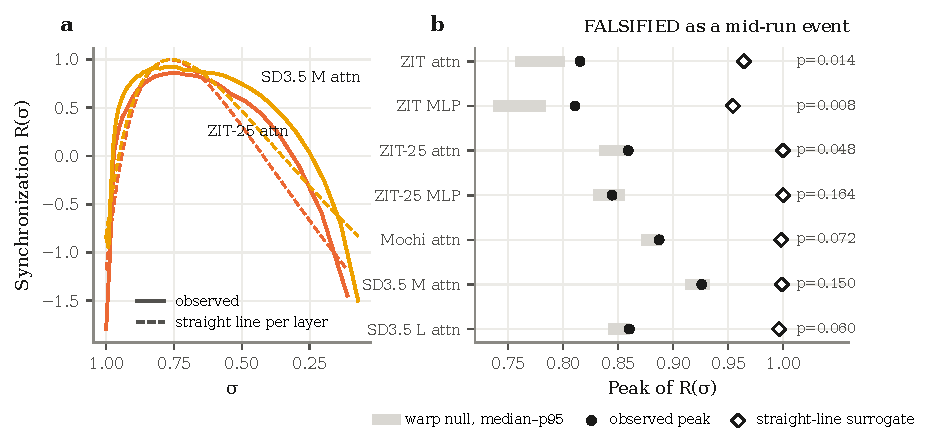
\includegraphics[width=\linewidth]{I-F12_sync_falsification}
 \caption{The historical synchronization peak is not a mid-run event. \textbf{(a)} Cross-layer order parameter $R(\sigma)$ of the population-mean field: observed against a per-layer straight-line surrogate (\TT{} and SD3.5\,M attention). The straight-line surrogate reaches a higher peak (1.00 vs 0.86; 1.00 vs 0.93). \textbf{(b)} Observed $R$ peak (0.81--0.93) against the monotone-warp null (median to p95, 500 draws) and the straight-line surrogate for seven channels: the straight-line surrogate exceeds the observed peak in 7/7; the warp null matches it ($p > 0.05$) in 4/7. The warp null is beaten only in ZIT attention and MLP ($p = 0.014$, $0.008$) and, marginally, \TT{} attention ($p = 0.048$). FALSIFIED as a mid-run synchronization event.}
 \label{fig:sync}
\end{figure}

\section{Analyzer instrument notes}\label{app:analyzer}
The layer-axis results use the CoS-PAFS Live Analyzer v3 (SHA-256 prefix \texttt{4089062551a3c900}) without modification. Four behaviours matter when it is applied to diffusion telemetry:
\begin{itemize}
 \item Its mean-profile, interval and ratio tools keep only rows with token type \texttt{generated}, so they return nothing on diffusion rows (type \texttt{step}); they were built for the language-model corpus. The layer-flow measurement on diffusion data is the dashboard's $\beta$-layer view.
 \item When a file contains both attention and MLP rows, most views average them per (layer, step) cell. Pooled Z-Image channels then show a single crossing.
 \item A header-less CSV is silently dropped by the loader. One Mochi CFG 4.5 domain file (73{,}152 rows) is affected, so Mochi CFG 4.5 results cover 9 of 10 domains; every Mochi CFG 4.5 number and figure panel in both papers inherits this coverage, and none of them enters the related--unrelated split or a lineage value. A loader for archive analysis should fail on such files instead.
 \item The Turbo archive includes four auxiliary 100-step generations, which enter step-axis views up to step 99.
\end{itemize}

\section{Estimator sensitivity}\label{app:estimators}
\begin{table}[htbp]
\centering\small
\caption{$\sigma_{50}$ and relative onset against sample size (SD3.5 Medium archive, branch-mean).}
\begin{tabular}{lcccc}
\toprule
Prompts $\times$ seeds & $n$ & $\sigma_{50}$ & Relative onset & Final $R^2$\\
\midrule
$30\times2$ & 60 & undefined (98\%) & 0.900 & 0.48\\
$60\times2$ & 120 & 0.720 & 0.867 & \\
$30\times4$ & 120 & 0.867 & 0.935 & \\
$120\times2$ & 240 & 0.843 & 0.915 & \\
$60\times4$ & 240 & 0.917 & 0.952 & \\
$120\times4$ & 480 & 0.936 & 0.956 & 0.89\\
\bottomrule
\end{tabular}
\end{table}
The fold partition alone moves $\sigma_{50}$ between $0.48$ and $0.63$ on one dataset. Simulated references for VR(4) on paths of the archive's length: random walk $0.816$--$0.828$, AR(0.8) $0.694$--$0.725$, i.i.d.\ $0.25$.

\section{Legacy instrument results}\label{app:legacy}
An early SD3.5 Medium suite (one prompt, 30 seeds per resolution, CFG 1, 100 steps, $512/768/1024$ pixels) and a CFG 1.0 versus 5.5 study at $256$ pixels were recorded with a capture path that substitutes an exponential-moving-average attention whenever it is registered. On those files depth profiles show a terminal rebound with four crossings, shape correlations of $0.989$--$0.996$ across resolutions, and a stable complex eigenpair of the local depth map. Because the instrument differs and the suite has a single prompt, these results are not used as evidence in this paper. The Round 3 captures at the same resolutions, with 60 prompts on the patched instrument, show $+,-,+,-$ rather than four crossings (\S\ref{sec:interventions}).

\section{Post hoc follow-ups on existing captures}\label{supp:posthoc}
After Round 18 was frozen, a sweep looked for analyses the existing captures allowed and the papers had not run. The checks were written down before they were run (\texttt{review/posthoc\_2026-11-10/\allowbreak PLAN.md}, SHA-256 prefix \texttt{27d056e4}, 2026-11-10 11:51 UTC) but after the data had been seen, so every result here is post hoc. The main value of the sweep is that the four Round 17 models, captured only for the tier controls, had never been used for the atlas: they are an untouched replication set for rules formed on the archive.

\begin{table}[htbp]
\centering\footnotesize
\caption{Archive rules replayed on the Round 17 models (PixArt-$\Sigma$, Cosmos-Predict2 2B: attention and MLP; SD3 Medium, SD3.5 Medium: attention; conditional branch, 60 prompts, seed 1001). Post hoc.}
\label{tab:posthocR17}
\begin{tabularx}{\linewidth}{@{}l>{\raggedright\arraybackslash}p{3.6cm}L@{}}
\toprule
Check & Rule replayed & Result\\
\midrule
RC34 & backbone (R11-5: PC1 $\ge0.70$, beats 999 depth-shift nulls) & 6 of 6 channels (PC1 $0.72$--$0.91$, rank $1.40$--$2.21$; unconditional branch 6 of 6)\\
RC35 & two components (B3, $\ge0.98$); autonomy (B4, $\Delta R^2\ge0.30$); anisotropy (B2/C1) & B3 5 of 6 (Cosmos MLP $0.967$); B4 6 of 6 ($0.51$--$0.67$); anisotropy fails in 6 of 6 (medians $0.057$--$0.114$)\\
RC36 & plateau onset in $[0.73,0.92]$ (B8) & 6 of 10 with Z1 and Z3; range $0.66$--$0.97$\\
RC37 & clock envelope signs (S4) & PixArt-$\Sigma$, Cosmos $+,+,-$ in both submodules; SD3 and SD3.5 Medium attention $+,+,+$ (all 100\% of bootstraps)\\
RC38 & layer-axis crossings & count changes with the row set in 5 of 6 channels (PixArt-$\Sigma$ MLP 4, 5 or 8): not stable\\
RC39 & first-state domain decoding & conditional branch 6 of 6 beat every baseline ($0.37$--$0.48$; scramble maximum $0.22$--$0.25$); unconditional at chance\\
RC40 & cross-model prompt geometry (S2) & unrelated attention pairs $0.04$--$0.49$ (median $0.29$), $96\%$ significant after removing text and length; PixArt-$\Sigma$$\leftrightarrow$Cosmos $0.33$--$0.44$\\
RC41 & text-to-latent handoff (R15-1) & 4 of 6; PixArt-$\Sigma$ reaches $0.5$ at step 4 of 20 instead of 2, and ends at $0.995$\\
\bottomrule
\end{tabularx}
\end{table}

\paragraph{What replicates and what narrows.} The backbone, the two-component triple, the non-autonomous depth step, first-state decoding and shared prompt geometry replicate on models that played no part in forming them. Three archive readings narrow: strong anisotropy of the uncentred second moment (it fails in all four models, so the C1 failure of the U-Net is not specific to convolution), the attention envelope $+,+,-$ (the SD3 family's conditional branch rises throughout; these captures used the card sampler rather than CoS-PAFS, Appendix~\ref{app:provenance}, which is a confound) and the plateau-onset window. The layer-axis crossing count is unstable, as RC29 found for most channels.

\paragraph{Row sets, the identity gate and decoding (RC43--RC46).} The identity gate separates Z-Image Base from Turbo through the caption rows: $0.655$ (attention) and $0.585$ (MLP) on all rows, $0.537$ and $0.904$ on caption rows, $0.945$ and $0.930$ on image rows and $0.959$ and $0.884$ centred, with split-half same weights at $0.997$ or more. On image rows the gate therefore reads the siblings in its undecided band, as it reads SD3.5 Large and Large Turbo ($0.986$, Round 18). First-state domain decoding holds on every row set of Z2 and the Round 11 Turbo session ($0.29$--$0.47$; RC45) and on the real Base ($0.54$/$0.46$; RC46).

\paragraph{The successor by depth half (RC47) and matrix regression (RC48).} SD3.5 Medium adds self-attention to its first 13 blocks (MMDiT-X). The successor tangent is $0.940$ on blocks 0--12 and $0.912$ on blocks 12--23 (same weights $0.990$ and $0.971$), so its shortfall from same weights is not concentrated in the changed blocks. A multiple regression of one model's prompt-distance matrix on another's gives the lineage pair $\beta=0.56$--$0.62$ and unrelated pairs $0.13$--$0.43$, every cell positive ($p\le0.01$), which restates the shared prompt geometry of \S\ref{sec:content}.

Three planned checks (seed estimators on the real Base, state against derivative alignment on the real lineage pair, and theme residuals for Base against Turbo) need older code ported to the new cubes and were not run.

\section{Round-8 review checks: the screen's limits}\label{supp:round8}
{\sloppy Post hoc checks RC53--RC56 (2026-11-11). The scripts are \texttt{rc53\_fpr\_inventory.py}, \texttt{rc54\_rc55\_round8.py} and \texttt{rc56\_grid12\_reconstruction.py} in the review-checks folder (\texttt{review/\allowbreak r15\_deep\_dive/\allowbreak review\_checks/}), with outputs in its \texttt{out/} folder. Summarised in \S\ref{sec:similarity} (``What the screen can and cannot claim'').\par}

\begin{table}[htbp]
\centering\scriptsize
\caption{Every depth-matched unrelated pair with an attention tangent on file (RC53). Native grid: one point per hooked layer (24 for these, so native and 24-point coincide except for PixArt-$\Sigma$$\leftrightarrow$Cosmos, 28 layers). Perm.\ p95: layer-order permutation; Surr.\ p95: smoothness-preserving surrogate (24-point grid). The ten capture pair-directions are five distinct model pairs of two types; none meets the lineage rule (p95 $+0.30$) on either grid; one lies above its permutation null on 24 points. Zero false positives among $k$ independent pairs give a one-sided 95\% upper bound of $1-0.05^{1/k}$ on the false-positive rate: $0.78$ ($k=2$), $0.45$ ($k=5$), $0.26$ ($k=10$).}
\label{tab:unrelinv}
\setlength\tabcolsep{2.5pt}
\begin{tabularx}{\linewidth}{@{}lLccccc@{}}
\toprule
Captures & Model pair & 24-pt & Perm. & Surr. & Native & Perm. (nat.)\\
\midrule
PixArt-$\Sigma$$\leftrightarrow$Cosmos 2B & PixArt-$\Sigma$ / Cosmos-Predict2 2B & 0.30 & 0.26 & 0.24 & 0.20 & 0.26\\
ACE turbo 6$\leftrightarrow$SD3.5 M (R17) & ACE-Step turbo / SD3.5 Medium & $-$0.07 & 0.32 & 0.26 & $-$0.07 & 0.35\\
ACE turbo 6$\leftrightarrow$SD3 M & ACE-Step turbo / SD3 Medium & $-$0.05 & 0.31 & 0.29 & $-$0.05 & 0.34\\
ACE turbo 6$\leftrightarrow$SD3.5 M (R11) & ACE-Step turbo / SD3.5 Medium & $-$0.09 & 0.33 & 0.26 & $-$0.09 & 0.36\\
ACE Base$\leftrightarrow$SD3.5 M (R17) & ACE-Step Base / SD3.5 Medium & $-$0.10 & 0.29 & 0.26 & $-$0.10 & 0.33\\
ACE Base$\leftrightarrow$SD3 M & ACE-Step Base / SD3 Medium & $-$0.06 & 0.30 & 0.34 & $-$0.06 & 0.33\\
ACE Base$\leftrightarrow$SD3.5 M (R11) & ACE-Step Base / SD3.5 Medium & $-$0.11 & 0.30 & 0.27 & $-$0.11 & 0.34\\
ACE turbo 8$\leftrightarrow$SD3.5 M (R17) & ACE-Step turbo / SD3.5 Medium & $-$0.16 & 0.34 & 0.29 & $-$0.16 & 0.37\\
ACE turbo 8$\leftrightarrow$SD3 M & ACE-Step turbo / SD3 Medium & $-$0.15 & 0.34 & 0.34 & $-$0.15 & 0.38\\
ACE turbo 8$\leftrightarrow$SD3.5 M (R11) & ACE-Step turbo / SD3.5 Medium & $-$0.17 & 0.36 & 0.30 & $-$0.17 & 0.37\\
\bottomrule
\end{tabularx}
\end{table}

\begin{table}[htbp]
\centering\scriptsize\setlength\tabcolsep{2pt}
\caption{The tangent by depth frequency (RC54, native grid $n$). Each state's depth differences are expanded in an orthonormal DCT-II basis along depth; the cosine is recomputed on the low ($k<(n-1)/4$), middle and high ($k\ge(n-1)/2$) coefficients and on the lowest 11, the most a 12-point grid can hold. Band permutation-null p95 in parentheses (300 draws). Upper energy: share of the first model's difference energy in the high band. The full-band cosine equals the native tangent.}
\label{tab:bands}
\begin{tabularx}{\linewidth}{@{}>{\raggedright\arraybackslash}p{1.9cm}Lcccccccc@{}}
\toprule
Relation & Pair & Sub & $n$ & Native & Low & Middle & High & 12-pt & Upper $E$\\
\midrule
same weights, sessions & Z3$\leftrightarrow$ZIT & attn & 30 & 0.99 & 0.98 (0.35) & 0.99 (0.45) & 0.99 (0.31) & 0.99 (0.42) & 0.66\\
same weights, sessions & Z3$\leftrightarrow$ZIT & mlp & 30 & 0.99 & 0.99 (0.36) & 0.99 (0.36) & 0.99 (0.29) & 0.99 (0.30) & 0.70\\
same weights, sessions & SD3.5 M (R17)$\leftrightarrow$SD3.5 M (R11) & attn & 24 & 0.98 & 0.99 (0.70) & 0.98 (0.44) & 0.97 (0.31) & 0.99 (0.50) & 0.41\\
same weights, sessions & ACE turbo 8$\leftrightarrow$ACE turbo 6 & attn & 24 & 0.92 & 0.83 (0.55) & 0.89 (0.48) & 0.92 (0.39) & 0.88 (0.46) & 0.89\\
same weights, sessions & SD3.5 L (R18)$\leftrightarrow$SD3.5 L (archive) & attn & 38 & 1.00 & 1.00 (0.49) & 0.99 (0.45) & 1.00 (0.38) & 1.00 (0.44) & 0.90\\
same weights, run & PixArt-$\Sigma$$\leftrightarrow$PixArt-$\Sigma$ uncond & attn & 28 & 1.00 & 0.99 (0.40) & 1.00 (0.43) & 1.00 (0.27) & 0.99 (0.35) & 0.67\\
successor & SD3 M$\leftrightarrow$SD3.5 M (R17) & attn & 24 & 0.93 & 0.96 (0.68) & 0.90 (0.42) & 0.91 (0.35) & 0.94 (0.48) & 0.46\\
distillation, documented & SD3.5 L (R18)$\leftrightarrow$SD3.5 L Turbo & attn & 38 & 0.90 & 0.94 (0.45) & 0.74 (0.44) & 0.91 (0.38) & 0.91 (0.43) & 0.90\\
distillation & ACE Base$\leftrightarrow$ACE turbo 8 & attn & 24 & 0.79 & 0.67 (0.55) & 0.72 (0.45) & 0.81 (0.34) & 0.65 (0.36) & 0.91\\
distillation & ACE Base$\leftrightarrow$ACE turbo 8 & mlp & 24 & 0.59 & 0.73 (0.53) & 0.74 (0.46) & 0.46 (0.23) & 0.74 (0.46) & 0.55\\
sibling & Z1 (Base)$\leftrightarrow$ZIT & attn & 30 & 0.55 & 0.65 (0.65) & 0.78 (0.51) & 0.46 (0.33) & 0.67 (0.52) & 0.65\\
sibling & Z1 (Base)$\leftrightarrow$ZIT & mlp & 30 & 0.77 & 0.82 (0.38) & 0.59 (0.34) & 0.80 (0.29) & 0.78 (0.27) & 0.67\\
unrelated & PixArt-$\Sigma$$\leftrightarrow$Cosmos 2B & attn & 28 & 0.20 & 0.66 (0.54) & 0.36 (0.49) & 0.01 (0.34) & 0.56 (0.41) & 0.67\\
unrelated & PixArt-$\Sigma$$\leftrightarrow$Cosmos 2B & mlp & 28 & 0.57 & 0.90 (0.47) & 0.41 (0.33) & 0.28 (0.24) & 0.78 (0.32) & 0.21\\
unrelated, cross-modal & ACE Base$\leftrightarrow$SD3.5 M (R17) & attn & 24 & $-$0.10 & 0.58 (0.50) & $-$0.22 (0.43) & $-$0.25 (0.39) & 0.35 (0.39) & 0.91\\
unrelated, cross-modal & ACE turbo 8$\leftrightarrow$SD3 M & attn & 24 & $-$0.15 & 0.36 (0.51) & $-$0.20 (0.49) & $-$0.25 (0.45) & 0.17 (0.41) & 0.89\\
unrelated, cross-modal & ACE turbo 6$\leftrightarrow$SD3.5 M (R11) & attn & 24 & $-$0.09 & 0.46 (0.52) & $-$0.25 (0.48) & $-$0.18 (0.37) & 0.18 (0.42) & 0.89\\
\bottomrule
\end{tabularx}
\end{table}

\begin{table}[htbp]
\centering\scriptsize
\caption{MLP tangent variants on the pairs with row-split captures (RC55, native grid, 300-draw nulls). Image rows equal all rows for PixArt-$\Sigma$ and Cosmos, whose hooks read image tokens only. End trim: first and last hooked layer removed.}
\label{tab:mlpvar}
\begin{tabularx}{\linewidth}{@{}Llllcccc@{}}
\toprule
Relation & Pair & Statistic & End trim & $n$ & Tangent & Perm.\ p95 & Surr.\ p95\\
\midrule
sibling & Z2 (Base)$\leftrightarrow$Turbo R11 & all & no & 30 & 0.77 & 0.21 & 0.37\\
sibling & Z2 (Base)$\leftrightarrow$Turbo R11 & all & yes & 28 & 0.79 & 0.22 & 0.39\\
sibling & Z2 (Base)$\leftrightarrow$Turbo R11 & image & no & 30 & 0.74 & 0.21 & 0.33\\
sibling & Z2 (Base)$\leftrightarrow$Turbo R11 & image & yes & 28 & 0.80 & 0.22 & 0.35\\
sibling & Z2 (Base)$\leftrightarrow$Turbo R11 & centred & no & 30 & 0.52 & 0.17 & 0.25\\
sibling & Z2 (Base)$\leftrightarrow$Turbo R11 & centred & yes & 28 & 0.50 & 0.15 & 0.22\\
sibling & Z2 (Base)$\leftrightarrow$Turbo R11 & top8 removed & no & 30 & 0.51 & 0.20 & 0.27\\
sibling & Z2 (Base)$\leftrightarrow$Turbo R11 & top8 removed & yes & 28 & 0.70 & 0.24 & 0.34\\
unrelated & PixArt-$\Sigma$$\leftrightarrow$Cosmos 2B & all & no & 28 & 0.57 & 0.17 & 0.29\\
unrelated & PixArt-$\Sigma$$\leftrightarrow$Cosmos 2B & all & yes & 26 & 0.39 & 0.21 & 0.23\\
unrelated & PixArt-$\Sigma$$\leftrightarrow$Cosmos 2B & image & no & 28 & 0.57 & 0.17 & 0.29\\
unrelated & PixArt-$\Sigma$$\leftrightarrow$Cosmos 2B & image & yes & 26 & 0.39 & 0.21 & 0.23\\
unrelated & PixArt-$\Sigma$$\leftrightarrow$Cosmos 2B & centred & no & 28 & 0.27 & 0.21 & 0.21\\
unrelated & PixArt-$\Sigma$$\leftrightarrow$Cosmos 2B & centred & yes & 26 & 0.26 & 0.18 & 0.16\\
unrelated & PixArt-$\Sigma$$\leftrightarrow$Cosmos 2B & top8 removed & no & 28 & 0.76 & 0.15 & 0.31\\
unrelated & PixArt-$\Sigma$$\leftrightarrow$Cosmos 2B & top8 removed & yes & 26 & 0.55 & 0.21 & 0.26\\
same weights, run & PixArt-$\Sigma$$\leftrightarrow$PixArt-$\Sigma$ uncond & all & no & 28 & 1.00 & 0.22 & 0.39\\
same weights, run & PixArt-$\Sigma$$\leftrightarrow$PixArt-$\Sigma$ uncond & all & yes & 26 & 1.00 & 0.23 & 0.37\\
same weights, run & PixArt-$\Sigma$$\leftrightarrow$PixArt-$\Sigma$ uncond & image & no & 28 & 1.00 & 0.22 & 0.39\\
same weights, run & PixArt-$\Sigma$$\leftrightarrow$PixArt-$\Sigma$ uncond & image & yes & 26 & 1.00 & 0.23 & 0.37\\
same weights, run & PixArt-$\Sigma$$\leftrightarrow$PixArt-$\Sigma$ uncond & centred & no & 28 & 0.99 & 0.19 & 0.32\\
same weights, run & PixArt-$\Sigma$$\leftrightarrow$PixArt-$\Sigma$ uncond & centred & yes & 26 & 0.94 & 0.15 & 0.34\\
same weights, run & PixArt-$\Sigma$$\leftrightarrow$PixArt-$\Sigma$ uncond & top8 removed & no & 28 & 1.00 & 0.17 & 0.35\\
same weights, run & PixArt-$\Sigma$$\leftrightarrow$PixArt-$\Sigma$ uncond & top8 removed & yes & 26 & 1.00 & 0.23 & 0.36\\
\bottomrule
\end{tabularx}
\end{table}

\begin{table}[htbp]
\centering\scriptsize\setlength\tabcolsep{2pt}
\caption{Reconstruction of the 12-point tangent from native-grid depth frequencies (RC56). 12-pt: the tangent after linear interpolation of the native profile onto 12 points. Ideal LP: the same after removing, before interpolation, every depth-cosine component of the profile that 12 points cannot represent ($k\ge11$). Band: the RC54 12-point band of the native differences (Table~\ref{tab:bands}). Folded: percentage of the 12-point difference energy contributed by the removed components, which linear interpolation folds back into the represented ones. An ideal low-pass filter would give 12-pt = Ideal LP and Folded = 0.}
\label{tab:recon12}
\begin{tabularx}{\linewidth}{@{}>{\raggedright\arraybackslash}p{1.9cm}Lccccccc@{}}
\toprule
Relation & Pair & Sub & $n$ & Native & 12-pt & Ideal LP & Band & Folded (\%)\\
\midrule
same weights, sessions & Z3$\leftrightarrow$ZIT & attn & 30 & 0.99 & 0.99 & 0.98 & 0.99 & 35\\
same weights, sessions & Z3$\leftrightarrow$ZIT & mlp & 30 & 0.99 & 0.99 & 0.99 & 0.99 & 21\\
same weights, sessions & SD3.5 M (R17)$\leftrightarrow$SD3.5 M (R11) & attn & 24 & 0.98 & 0.98 & 0.99 & 0.99 & 8\\
same weights, sessions & ACE turbo 8$\leftrightarrow$ACE turbo 6 & attn & 24 & 0.92 & 0.90 & 0.87 & 0.88 & 33\\
same weights, sessions & SD3.5 L (R18)$\leftrightarrow$SD3.5 L (archive) & attn & 38 & 1.00 & 0.99 & 1.00 & 1.00 & 27\\
same weights, run & PixArt-$\Sigma$$\leftrightarrow$PixArt-$\Sigma$ uncond & attn & 28 & 1.00 & 0.99 & 0.99 & 0.99 & 28\\
successor & SD3 M$\leftrightarrow$SD3.5 M (R17) & attn & 24 & 0.93 & 0.93 & 0.96 & 0.94 & 10\\
distillation, documented & SD3.5 L (R18)$\leftrightarrow$SD3.5 L Turbo & attn & 38 & 0.90 & 0.96 & 0.97 & 0.91 & 27\\
distillation & ACE Base$\leftrightarrow$ACE turbo 8 & attn & 24 & 0.79 & 0.51 & 0.67 & 0.65 & 23\\
distillation & ACE Base$\leftrightarrow$ACE turbo 8 & mlp & 24 & 0.59 & 0.59 & 0.53 & 0.74 & 14\\
sibling & Z1 (Base)$\leftrightarrow$ZIT & attn & 30 & 0.55 & 0.70 & 0.66 & 0.67 & 16\\
sibling & Z1 (Base)$\leftrightarrow$ZIT & mlp & 30 & 0.77 & 0.81 & 0.84 & 0.78 & 20\\
unrelated & PixArt-$\Sigma$$\leftrightarrow$Cosmos 2B & attn & 28 & 0.20 & 0.60 & 0.65 & 0.56 & 28\\
unrelated & PixArt-$\Sigma$$\leftrightarrow$Cosmos 2B & mlp & 28 & 0.57 & 0.80 & 0.79 & 0.78 & 6\\
unrelated, cross-modal & ACE Base$\leftrightarrow$SD3.5 M (R17) & attn & 24 & $-$0.10 & 0.56 & 0.57 & 0.35 & 23\\
unrelated, cross-modal & ACE turbo 8$\leftrightarrow$SD3 M & attn & 24 & $-$0.15 & 0.62 & 0.53 & 0.17 & 33\\
unrelated, cross-modal & ACE turbo 6$\leftrightarrow$SD3.5 M (R11) & attn & 24 & $-$0.09 & 0.56 & 0.49 & 0.18 & 35\\
\bottomrule
\end{tabularx}
\end{table}

\section{Capture cost}\label{supp:cost}
Per hook and sampling step the capture node forms the $D\times D$ Gram matrix $X^\top X/N$ in single precision and takes its symmetric eigendecomposition (\texttt{torch.linalg.eigvalsh}), a cost of order $ND^2+D^3$ on the GPU, and stores three numbers plus metadata, so storage grows with layers $\times$ steps $\times$ generations, not with $N$ or $D$. The full passive archive (six diffusion campaigns and the language-model controls) is about 0.7\,GB of CSV. Wall-clock overhead was not benchmarked systematically; for the largest image model here (SD3.5 Large, $D=2432$, 38 layers, 28 steps, one hook) it is one eigendecomposition of a $2432\times2432$ matrix per layer and step. Routine auditing would only need the first sampling state (the identity gate) or a few states, which is a small fraction of a full capture. A benchmark of overhead against model size and resolution is a Mode-III item.

\section{Supplementary figures}\label{app:supp}
\begin{figure}[h]
 \centering
 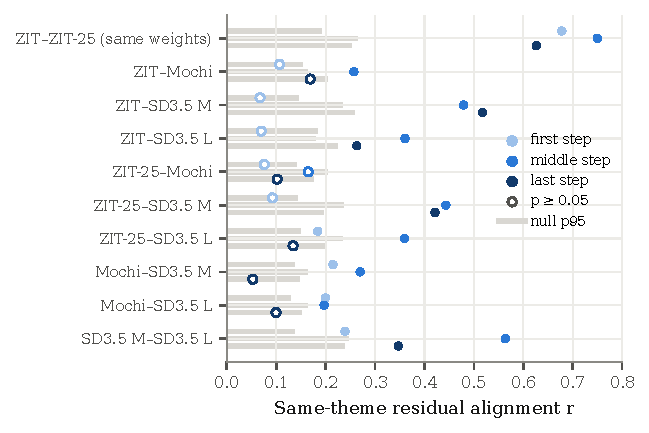
\includegraphics[width=\linewidth]{I-S1_theme_residual}
 \caption{Same-theme residual alignment after each model/time backbone is removed, for all model pairs at the first, middle and last step. Bars show the theme-label permutation null p95. The two Turbo campaigns (same weights): 0.63--0.75 at every step, the strongest; at the first step every other pair is $\le 0.24$; by the middle step unrelated pairs reach up to 0.48, and up to 0.52 by the last step (ZIT$\leftrightarrow$SD3.5\,M). Theme alignment is strongest for the same weights at every step and specific to them only at the first step.}
 \label{fig:S1}
\end{figure}

\begin{figure}[h]
 \centering
 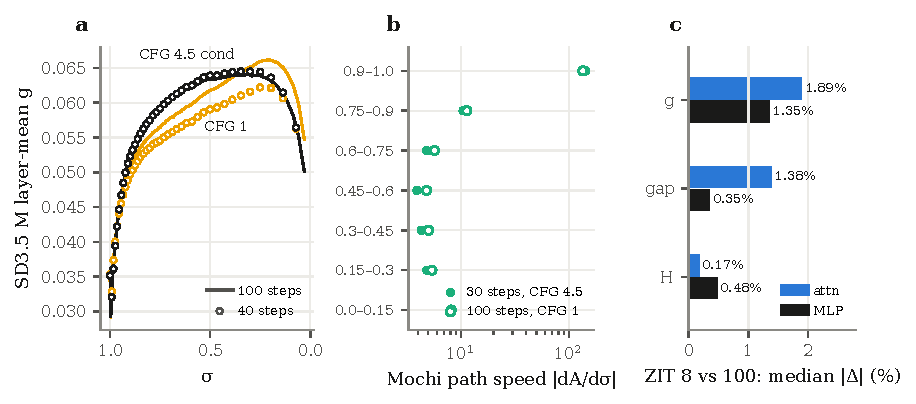
\includegraphics[width=\linewidth]{I-S2_stepcount_controls}
 \caption{Per-$\sigma$ geometry changes by at most 2--3\% between 8/40 and 100 steps. \textbf{(a)} SD3.5\,M, one prompt, explicit cond branch: layer-mean attention $g(\sigma)$ at 40 (markers) and 100 steps (lines), CFG\,1 and CFG\,4.5. The same-prompt 40$\to$100 shift is 0.033 at CFG\,1 (seed-split null p95 0.027, $p = 0.023$) and 0.007 at CFG\,4.5 (p95 0.022, $p = 0.70$). \textbf{(b)} Mochi 30 vs 100 steps: path speed by $\sigma$ band (ratio 0.81--1.06). The two arms also differ in CFG (4.5 vs 1). \textbf{(c)} ZIT 8 vs 100 steps at matched $\sigma$: median relative difference of $g$ (1.9\% attn / 1.4\% MLP), gap (1.4\% / 0.4\%) and $H$ (0.2\% / 0.5\%). The 100-step set contains only 4 generations.}
 \label{fig:S2}
\end{figure}

\begin{figure}[h]
 \centering
 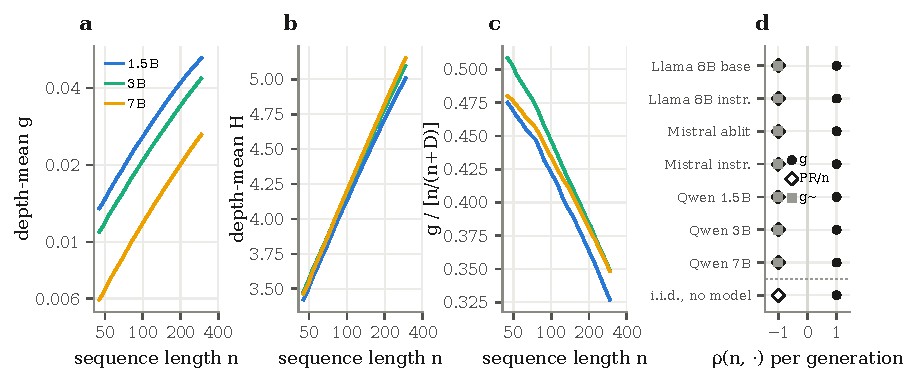
\includegraphics[width=\linewidth]{I-S3_qwen_context_clock}
 \caption{Why per-token phase claims for autoregressive models are not made. The v1 LLM capture re-encodes the full context at every token without a KV cache, so each logged value is a running statistic of a nested $n\times D$ matrix. \textbf{(a, b)} Depth-mean $g$ and $H$ of generated tokens against sequence length $n$ for Qwen2.5 1.5B/3B/7B (median per $n$ bin). \textbf{(c)} $g$ normalized by the finite-sample baseline $n/(n+D)$ remains monotone in $n$. \textbf{(d)} Median within-generation Spearman $\rho(n,\cdot)$ for all seven LLM captures: $\rho = 1.00$ for $g$ and $\le -0.999$ for PR$/n$ and $\tilde g$. The bottom row is a model-free reference (Round 9, preregistered): nested running statistics of i.i.d.\ Gaussian rows (180 simulations; isotropic, power-law and spiked spectra; $D=1536$ and $4096$) give the same $\rho$ without any network, so the monotonicity is a property of the capture. The Qwen multiscale $\beta$ "anomaly" therefore is a context-length clock, and it is demoted.}
 \label{fig:S3}
\end{figure}

\begin{figure}[h]
 \centering
 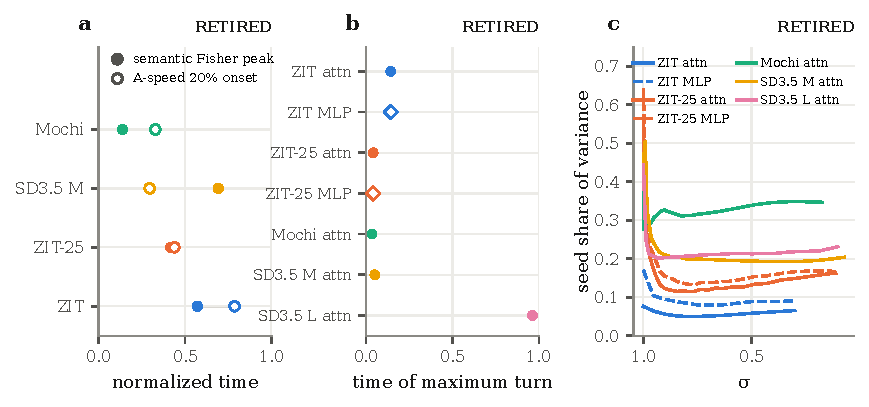
\includegraphics[width=\linewidth]{I-S4_negative_atlas}
 \caption{Retired claims. Every panel is marked RETIRED. \textbf{(a)} "The semantic decoder maximum is the universal C1 time": the smoothed semantic Fisher peak (0.14--0.69) does not track the A-speed 20\% onset (0.30--0.79) in normalized time (differences $-0.21$ to $+0.40$). \textbf{(b)} "Trajectory curvature gives a universal C1 detector": the time of the maximum turning angle falls in the early transient ($\tau \le 0.14$) in six of seven channels and at $\tau = 0.96$ in SD3.5\,L. \textbf{(c)} "Universal seed collapse": seed share of within-step variance along $\sigma$ (ANOVA). It ranges from 0.05--0.08 (ZIT attention) to a peak of 0.64 (25-step Turbo MLP, \TT{}), with no common collapse. The retired passive-susceptibility peak is not shown, because no per-channel values are stored.}
 \label{fig:S4}
\end{figure}

\begin{figure}[h]
 \centering
 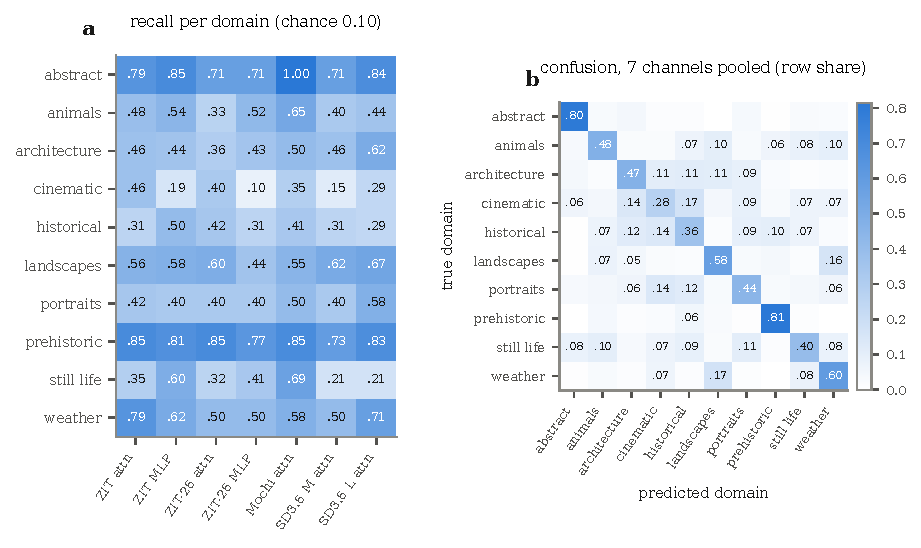
\includegraphics[width=\linewidth]{I-S5_domain_confusion}
 \caption{Which domains the first-state decoder recovers (descriptive). Same decoder, features and prompt-grouped folds as Fig.~\ref{fig:decode}a, with out-of-fold predictions. \textbf{(a)} Recall per domain for the seven archive channels (chance 0.10). Every cell is above chance except cinematic prompts in 25-step Turbo MLP (\TT{}; 0.10). Abstract (0.71--1.00) and prehistoric (0.73--0.85) prompts are recovered best, cinematic (0.10--0.46) and still-life prompts (0.21--0.69) worst. \textbf{(b)} Confusion matrix summed over the seven channels, as row shares; values below 0.05 are not printed. Errors spread over several domains rather than concentrating in one pair; the largest off-diagonal shares are landscapes$\leftrightarrow$weather (0.16, 0.17).}
 \label{fig:S5}
\end{figure}
